\chapter{ACCRETION DISKS}

The term \emph{accretion} comes from a Latin word \emph{accrescere} which literarily means \emph{become larger}, and in astronomy, we refer exactly to that process. That is the \emph{coming together and cohesion of matter under the influence of gravity to form larger bodies}. One could easily argue that it is one of the most fundamental processes in the universe. From the giant galaxies to the tiniest rocks floating around in the solar system. All the stars, planets, and all there is were smashed together by gravity at some point in the past. Atom by atom, piece by piece, to form larger and larger structures. Even the dinosaurs probably met their fate by a city-sized asteroid that accreted Earth some 65 million years ago. 

\section{Types of accreting systems}

Accretion is not only the mass moving and colliding but also energy taking different forms in the process. Depending on the nature of the accreting system and its central object, many types of radiation escape the swirling vortex of matter we call \emph{accretion disk}. If we sort accreting astrophysical systems based on their size and radiation power, we can classify them as follows.

\subsection{Active galactic nuclei (AGN) and Quasar}

As \emph{active galactic nucleus} (AGN), we refer to a central high-luminosity region containing a supermassive black hole in most galaxies' centers. The radiative power of the AGN is usually higher than that of the whole host galaxy, and the radiation characteristics indicate that stars are not the primary source of this radiation. Instead, mass accretion onto the central supermassive black hole is the more likely source of this excess non-stellar radiation. 

The main distinguishing characteristic of AGNs is whether they are \emph{radio loud} or \emph{radio quiet}, which depends on the existence of jets. By \emph{jets}, we mean relatively narrow streams of accreted mass ejected from the black hole in both directions, roughly colinear with its axis of rotation. These mass ejections can travel at relativistic speeds and reach thousands of light-years away from the source object. 

Figure \ref{fig:centaurus_a_multiwave} shows the Centaurus A (NGC 5128) galaxy with an active supermassive black hole in its center. This object is typical \emph{radio loud} AGN. We can see both the jets in the radio part of the spectrum and the accreted matter in other parts of the spectrum. For example, the galaxys' dust core is most apparent in visible light.

A particular sub-category of AGN is Quasars. The name \emph{Quasar} is a contraction of the phrase \emph{quasi-stellar radio source} because, in the 1950s, they were detected as radio sources of unknown physical characteristics and also in visible light as faint \emph{star-like} light sources. However, they are nothing like stars. These highly luminous objects are observed to the highest values of redshift. The current record holder for the most distant Quasar is the J0313-1806 detected at redshift $z = 7.64$ by \cite{wang2021}. 

Due to the extreme distance, it is impossible, at least with today's methods, to distinguish the active core (i.e., the supermassive black hole), whose mass can range from $10^6 M_{\odot}$ to $10^{9} M_{\odot}$. To this day, more than a million quasars have been discovered with the closest known Markarian 231 (UGC 8058) at 581 milion light-years away \cite{gaia2018}. 

\begin{figure}
    \centering
    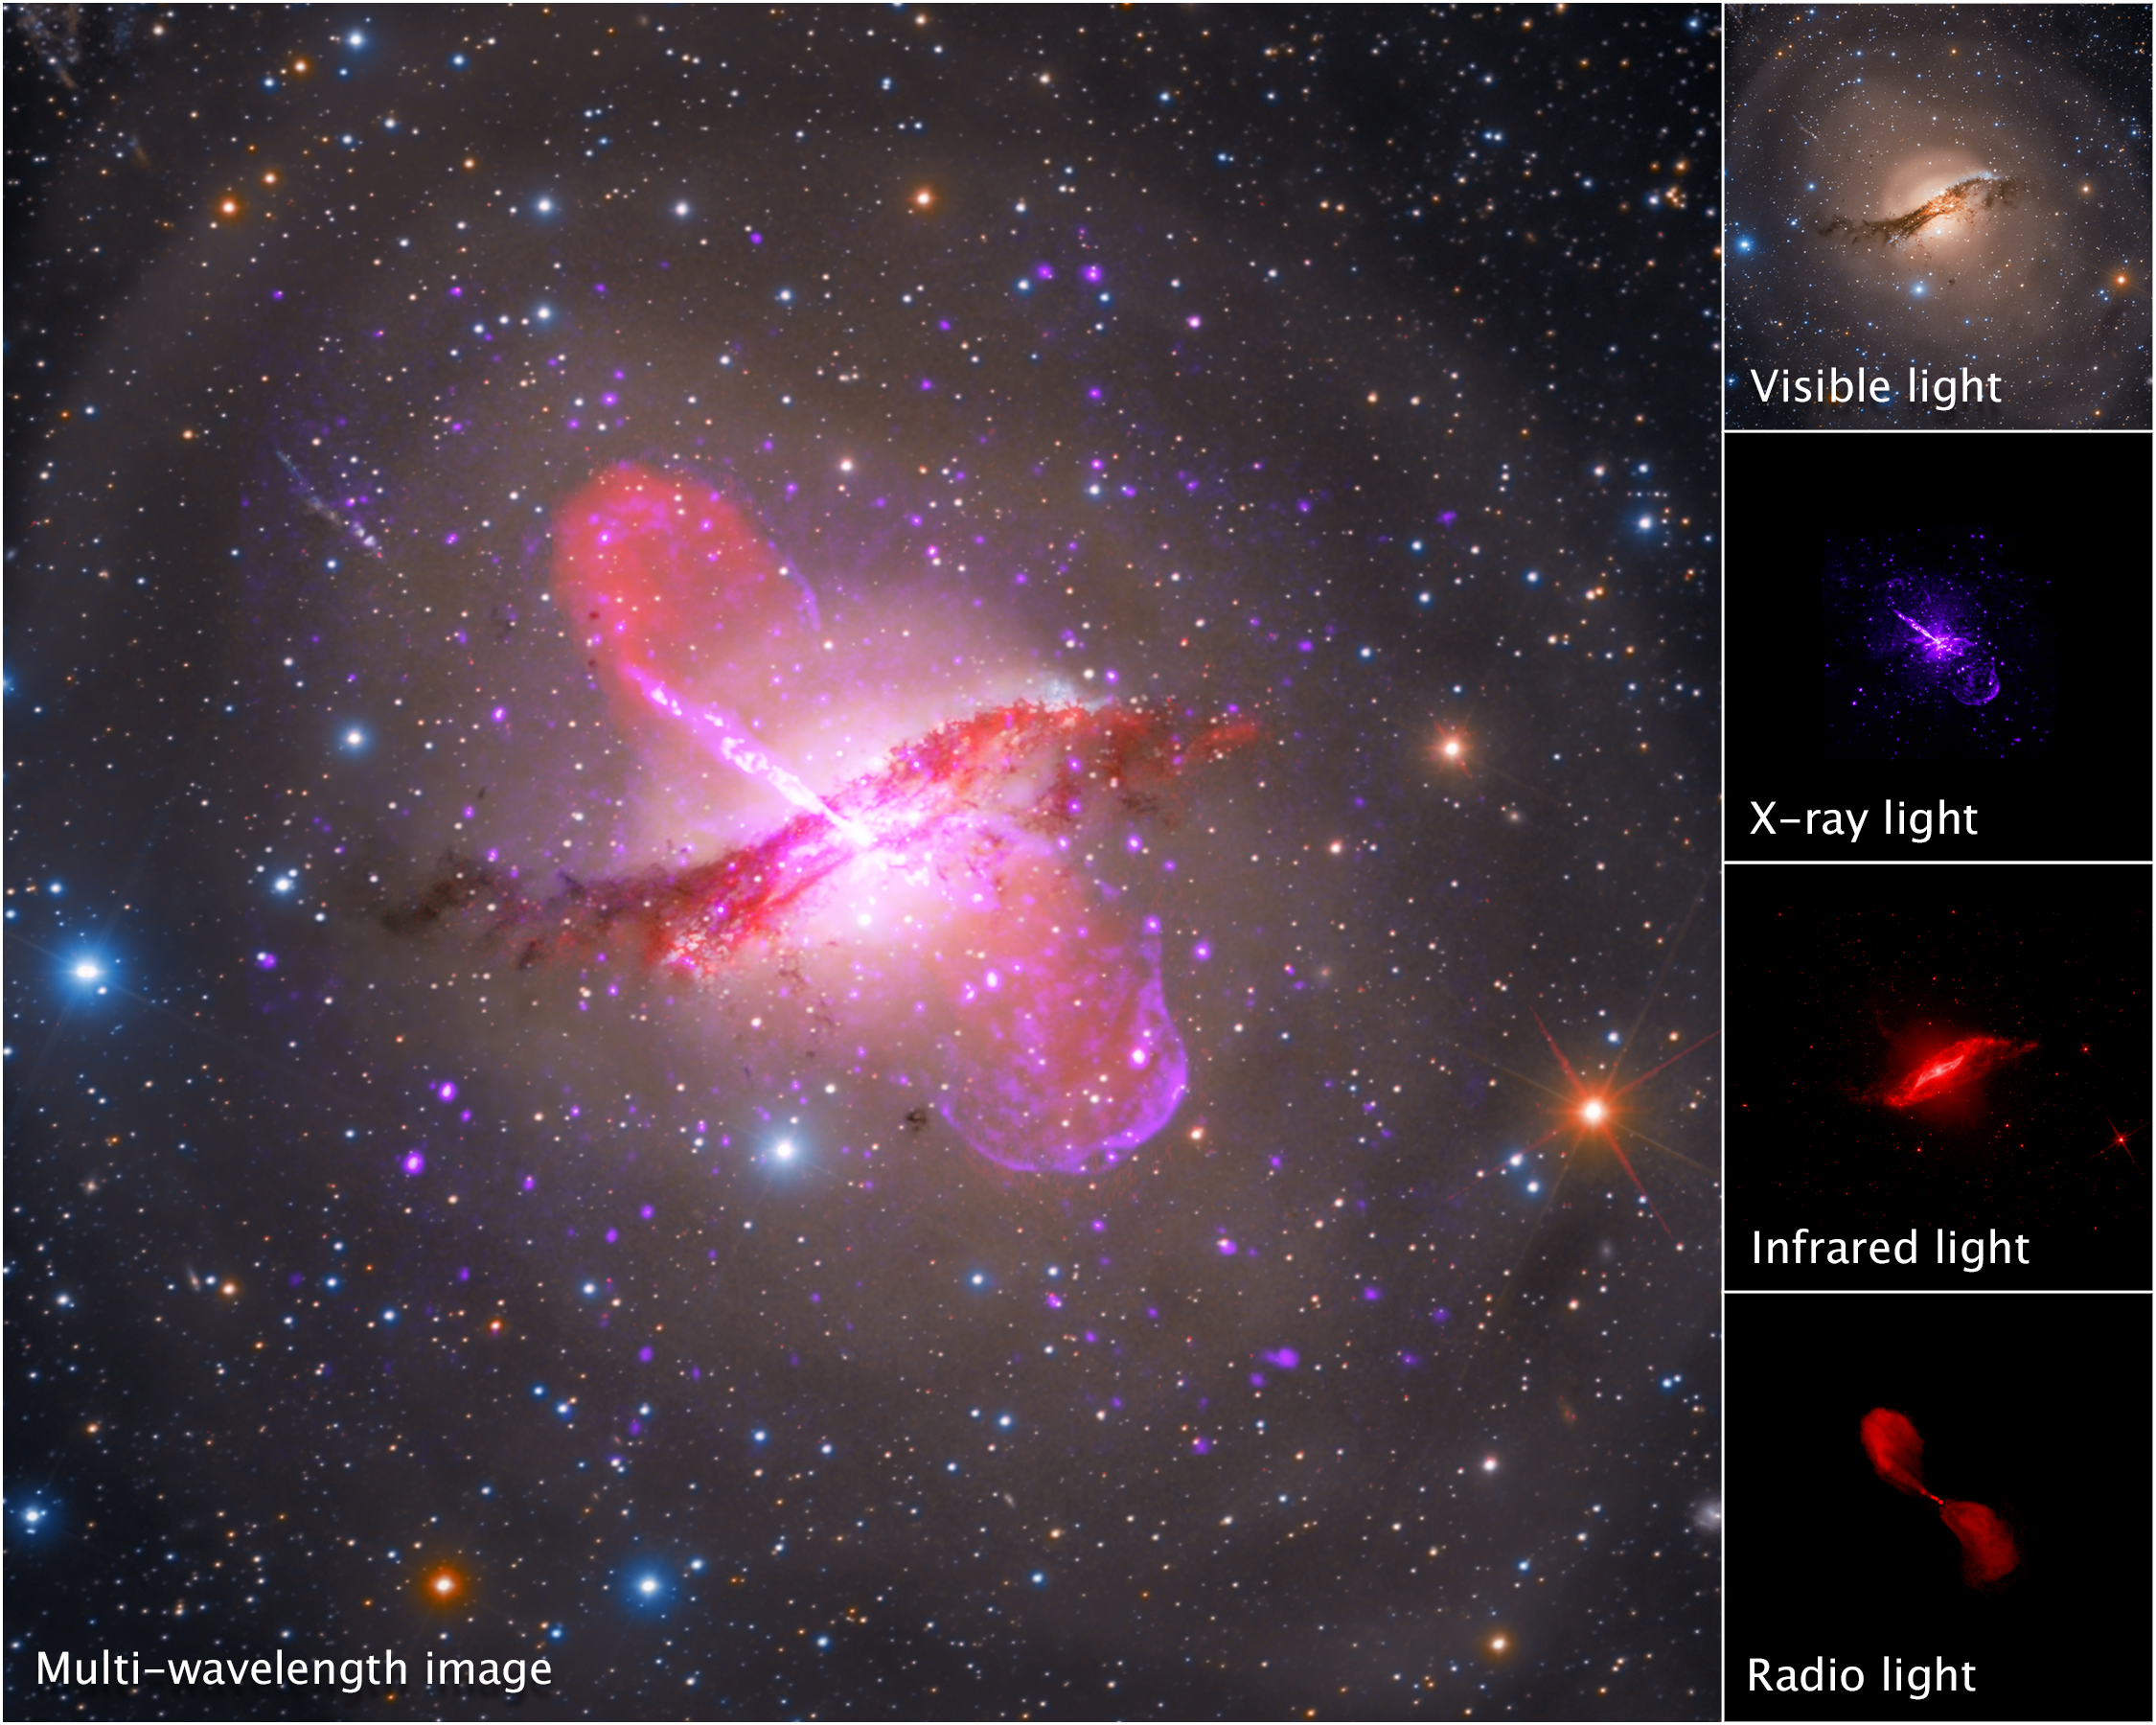
\includegraphics[width=\columnwidth]{img/multiwave_centaurus_a_agn.png}
    \caption{Multi-wavelength composition (left) and multiple narrow wavelengh observations (right) of Centaurus A. Taken from \cite{nasa_img_centaurus_a}}
    \label{fig:centaurus_a_multiwave}
\end{figure}

\subsection{X-ray binaries (XB)}

The main sequence star in orbit around a neutron star (NSB) or a black hole (BHB) is commonly referred to as a \emph{X-ray binary} (XRB). The gravitational potential of these systems is strong enough that the accreting matter produces energy output up to the X-rays. Based on the mass of the primary component (i.e., the accretor), this class of binary stars is also usually split between \emph{Low-mass X-ray binary} (LXRB) and \emph{High-mass X-ray binary} (HXRB). 

Most XRB objects go through periods of high activity when they emit twin jets at relativistic speed, not that dissimilar to those of AGN but at a smaller scale.

Suppose the accretor is the strongly magnetized young neutron star. In that case, the accretion disk is truncated by its magnetic field or not present at all, and the matter transfers onto the neutron star by \emph{column accretion}. 

\subsection{Young stellar objects (YSO)}
When a proto-star is formed from a collapsing molecular cloud, the gas and solid particles envelope forms a rotating protoplanetary accretion disk. Instabilities and self-gravity in the disk's body eventually lead to planets and other smaller objects forming. The proto-star is only detectable in infrared due to the relatively dense surrounding matter that obscures it.   

The YSO classification consists of five classes (0-IV) based on the infrared and visible spectral energy distribution. Class 0 is a collapsing molecular cloud. Classes I to III are YSO with a formed proto-planetary disk in various stages of evolution, and lastly, class IV refers to a fully formed zero-aged star. 

\subsection{Cataclysmic variables (CV)}

The Cataclysmic Variables (CV) are of particular interest to this study because our modeling efforts in the latter chapters are focused on generic CV systems. Unlike the LMXB or HMXB, where the primary component is either a black hole or neutron star, the accretor in CV is a White Dwarf (WD), and its companion is a late-type star. Due to its nature, this system has a relatively weaker gravitational potential; therefore, its radiation energy output is lower than that of the XRB.

CVs are comparable in size to planetary or Earth-Moon-like systems. The primary WD is a stellar core remnant composed of very dense electron-degenerate gas, and its size can be approximated by the \emph{mass-radius ratio} \cite{shapiro1983}

\begin{equation}
    r_{\textrm{in}} \sim M^{-1-3}_{\textrm{p}},
    \label{eq:mass_radius_ratio}
\end{equation}

where $M^{-1-3}_{\textrm{p}}$ represents the WD mass and $r_{in}$ its radius, which also corresponds to the inner boundary layer radius of the accretion disk.

The secondary component star fills its Roche lobe, and the overflowing matter falls onto the WD through the Langrangian point $L_1$. If the WD is not magnetized or weakly magnetized, the gas stream forms an accretion disk around the WD that eventually reaches its surface. In the case of strongly magnetized WD, the accretion disk is truncated or non-existent, and the magnetic field lines direct the accretion flow. 

Another important parameter of the CV binary system is its size, which is closely related to individual component masses and determines the accretion disk size because the disk's outer edge is constrained by the gravitational potential, namely the Langrangian $L_1$. The outer disk radius is calculated

\begin{equation}
    r_{out} = d \left[ \frac{M_{\textrm{s}}}{3(M_{\textrm{p}}+M_{\textrm{s}})} \right]^{1/3},
    \label{eq:disk_outher_radius}
\end{equation}

where $M_{\textrm{s}}$ represents the secondary components' mass and $d$ is the distance between the components. 
\subsection{Gamma ray bursts (GRB)}














\section[Shakura-Sunyaev $\alpha$-Disc model]{Shakura-Sunyaev $\alpha$-Disc model}
\begin{align}
\begin{split}
\Sigma 	&= 5.2 \alpha^{-4/5} \dot{M}^{7/10}_{16} m^{1/4}_1 R^{-3/4}_{10} f^{14/5}\ \mathrm{g\ cm^{-2}}, \\
H		&= 1.7 \times 10^8 \alpha^{-1/10} \dot{M}^{3/20}_{16} m^{-3/8}_1 R^{9/8}_{10} f^{3/5}\ \mathrm{cm}, \\
\rho		&= 3.1 \times 10^{-8} \alpha^{-7/10} \dot{M}^{11/20}_{16} m^{5/8}_1 R^{-15/8}_{10} f^{11/5}\ \mathrm{g\ cm^{-3}}, \\
T_c		&= 1.4 \times 10^4 \alpha^{-1/5} \dot{M}^{3/10}_{16} m^{1/4}_1 R^{-3/4}_{10} f^{6/5}\ \mathrm{K}, \\
\tau		&= 190 \alpha^{-4/5} \dot{M}^{1/5}_{16} f^{4/5}, \\
\nu		&= 1.8 \times 10^{14} \alpha^{4/5} \dot{M}^{3/10}_{16} m^{3/4}_1 R^{3/4}_{10} f^{6/5}\ \mathrm{cm^2\ s^{-1}},  \\
v_R		&= 2.7 \times 10^{14} \alpha^{4/5} \dot{M}^{3/10}_{16} m^{-1/4}_1 R^{-1/4}_{10} f^{-14/15}\ \mathrm{cm\ s^{-1}},  \\
\mathrm{with}\ f		&= \left[ 1 - \left( \frac{R_*}{R} \right)^{1/2} \right]^{1/4}. \\
\end{split}
\label{eq:alpha_model}
\end{align}
